\section{Бетатронное движение}
\textbf{Вопрос.} Как выглядит поперечное движение на том же кольце, где полость включена?

Амплитуда $A_x=\vAxmm$~мм, $\delta_m=\vdm$. Действие Куранта--Снайдера $J_x=\vJxCS$~м, $\beta_x=\vbetax$~м в точке наблюдения.

\begin{figure}[H]\centering
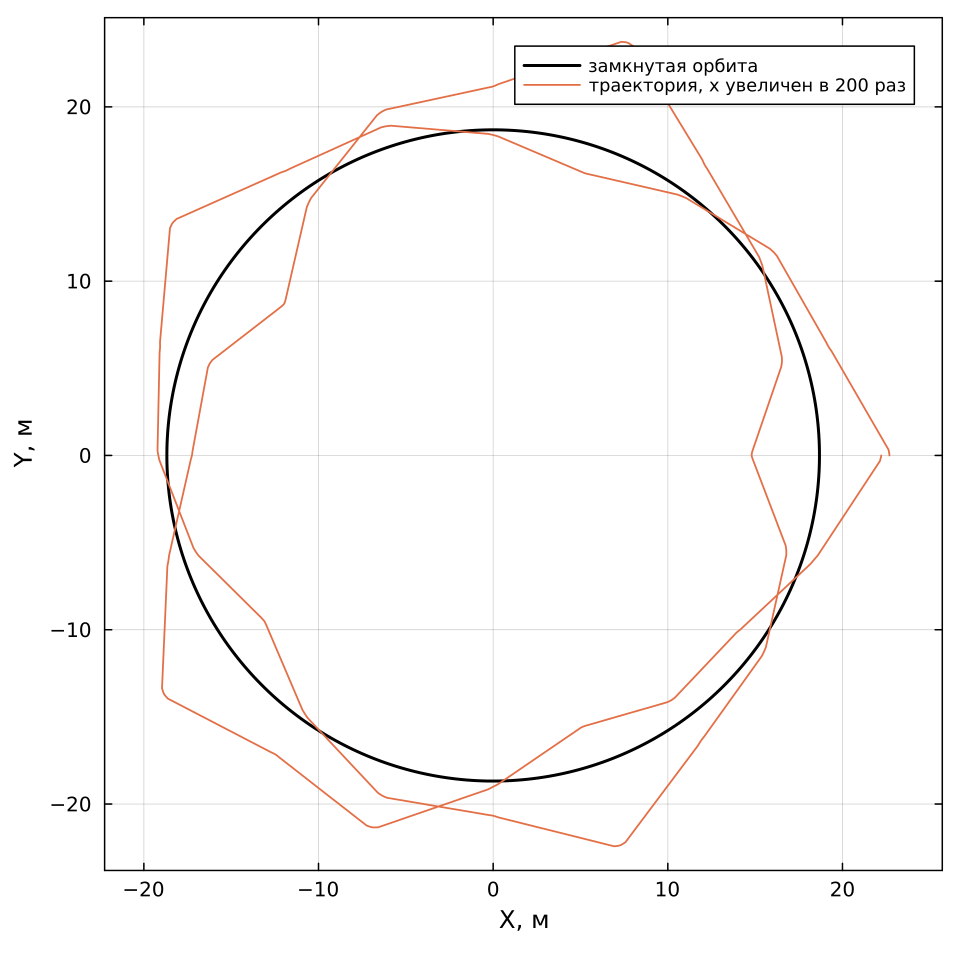
\includegraphics[width=0.72\textwidth]{figs/fig_04_ring.png}
\caption{Два оборота на плане кольца. Поперечное смещение увеличено в $\vxScale$ раз: иначе миллиметры на фоне $C=\vCirc$~м не видны. Полоса вокруг орбиты --- след бетатрона.}
\end{figure}

\begin{figure}[H]\centering
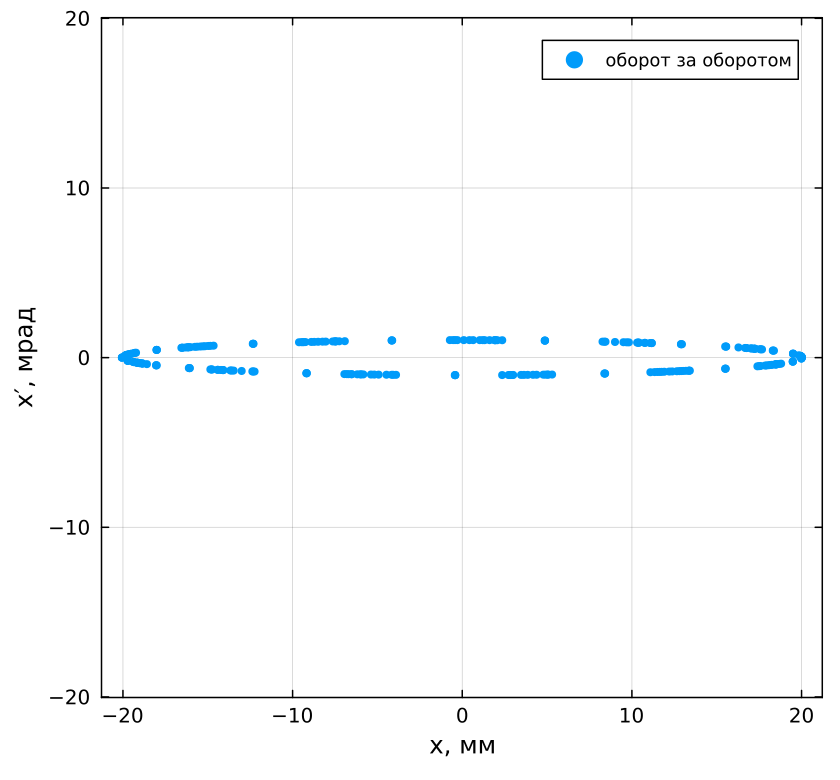
\includegraphics[width=0.62\textwidth]{figs/fig_04_ellipse.png}
\caption{Эллипс $(x,x')$ оборот за оборотом. ВЧ включён: эллипс медленно дышит из-за синхротрона через дисперсию.}
\end{figure}

\textbf{Вывод.} Бетатрон есть поверх синхротрона. Это то движение, которое ниже удлиняет путь.
